\documentclass[conference]{IEEEtran}
\IEEEoverridecommandlockouts

\usepackage{cite}
\usepackage{amsmath,amssymb,amsfonts}
\usepackage{algorithmic}
\usepackage{graphicx}
\usepackage{textcomp}
\usepackage{xcolor}
\usepackage{url}
\usepackage{babel}[portuguese]
\usepackage{cuted}
\usepackage{caption}
\usepackage{capt-of}

\begin{document}

\title{Visualização de Árvores de Decisão}

\author{\IEEEauthorblockN{Joel Perca}
\IEEEauthorblockA{\textit{FGV EMAp} \\
Rio de Janeiro, Brasil}
\and
\IEEEauthorblockN{Mariana Fernandes Rocha}
\IEEEauthorblockA{\textit{FGV EMAp} \\
Rio de Janeiro, Brasil}
\and
\IEEEauthorblockN{Paula Eduarda de Lima}
\IEEEauthorblockA{\textit{FGV EMAp} \\
Rio de Janeiro, Brasil}
}

\maketitle

\begin{strip}
  \centering
  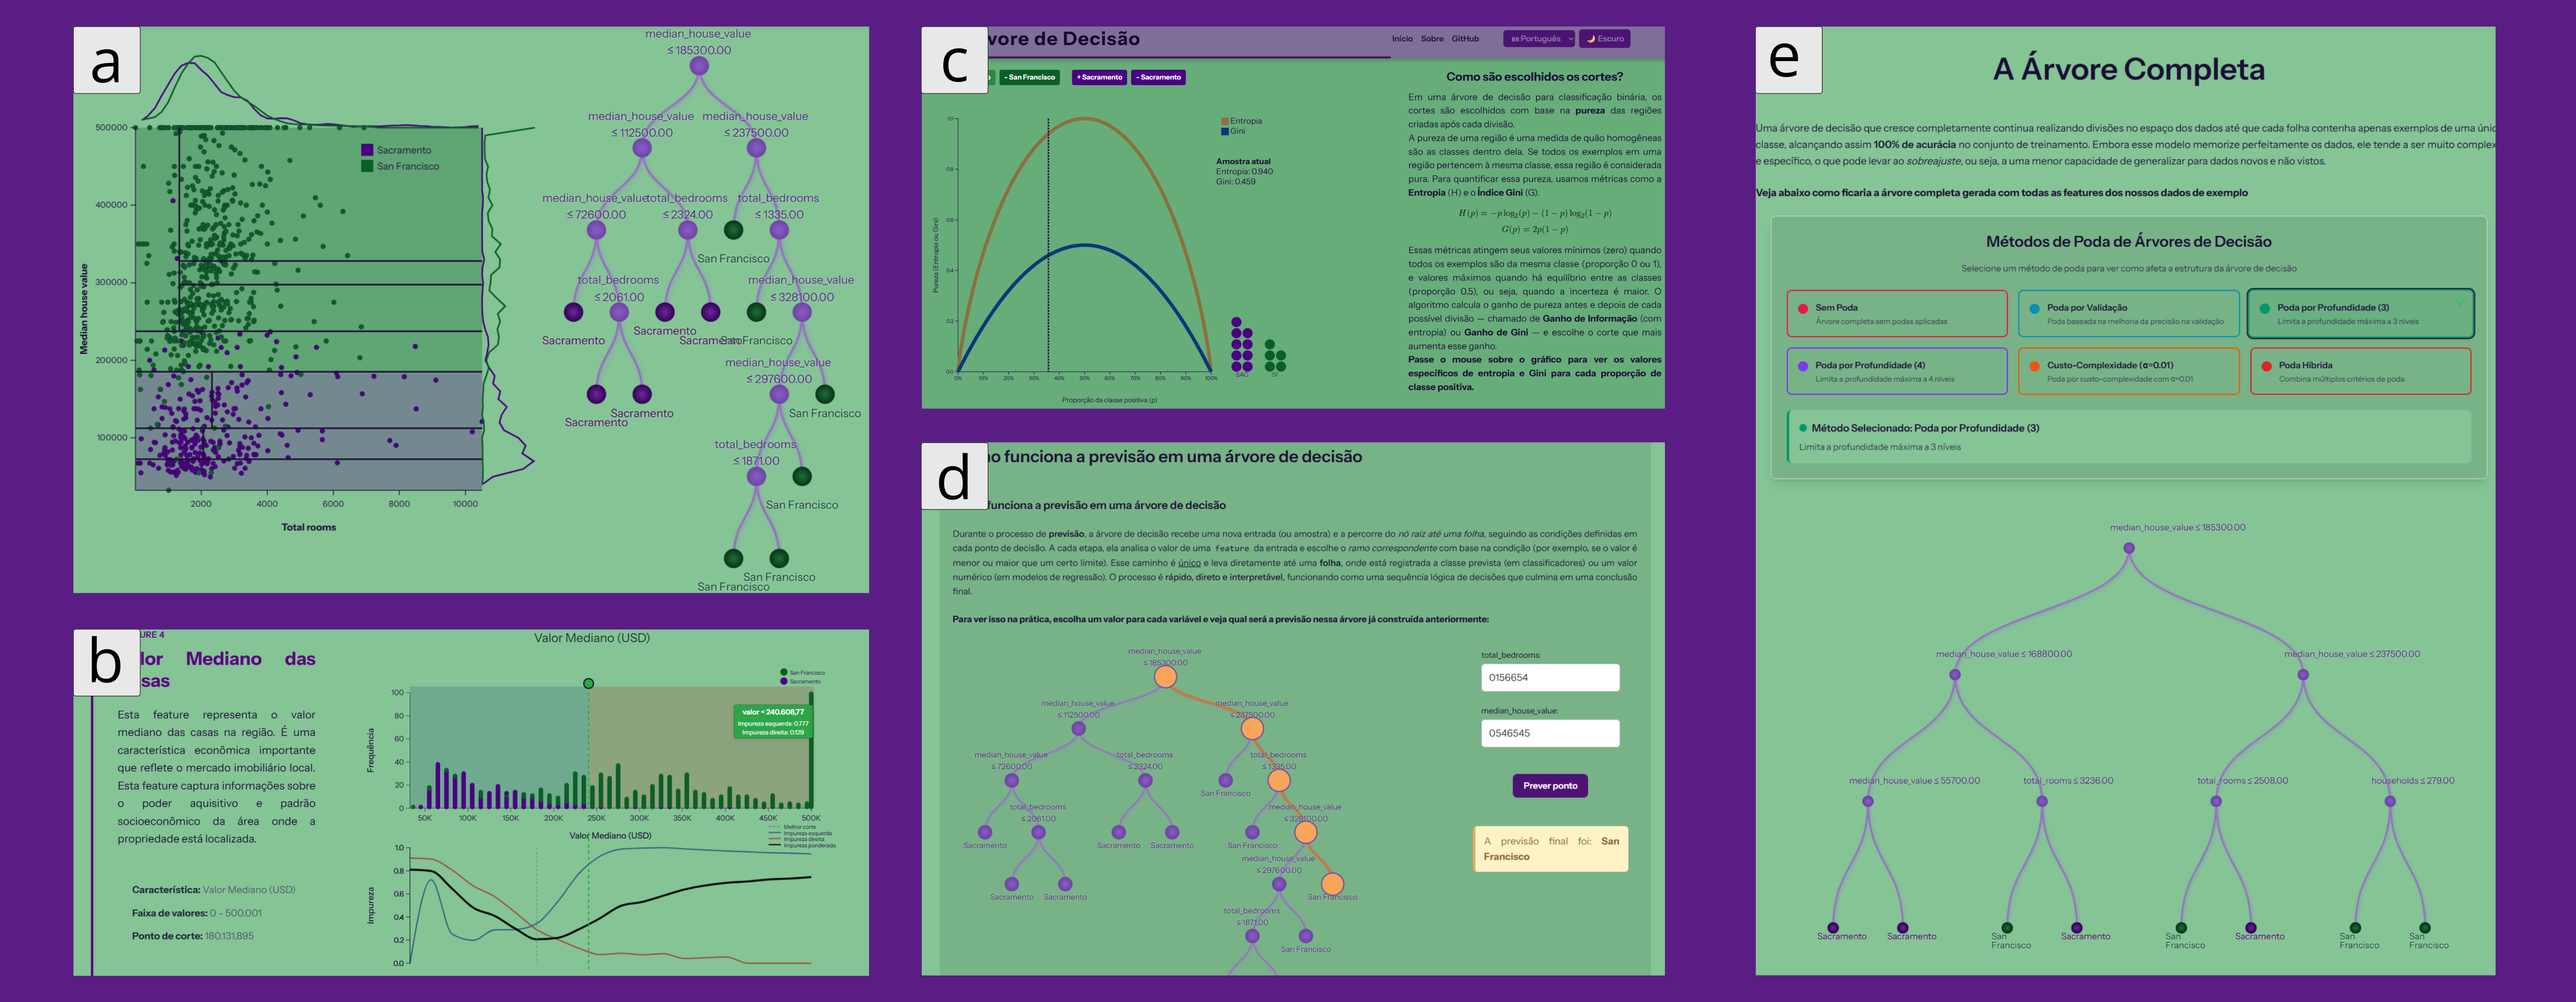
\includegraphics[width=\textwidth]{teaser.pdf.png}
  \captionof{figure}{Capturas das principais etapas da visualização interativa.
(a) Construção dinâmica da árvore de decisão e segmentação do espaço 2D dos dados.
(b) Análise univariada de variáveis com visualização dos pontos de corte.
(c) Visualização das métricas de impureza (Gini e Entropia) ao longo da proporção de classes.
(d) Simulação interativa de predição, com percurso visual da amostra pela árvore.
(e) Exibição da árvore completa e opções de poda, permitindo comparar diferentes métodos de simplificação da estrutura.}
  \label{fig:teaser}
\end{strip}


\begin{abstract}

Este projeto tem como objetivo principal ampliar a experiência prática no desenvolvimento, implementação e avaliação de métodos de visualização, abordando um problema concreto e propondo uma solução inovadora e criativa. O desafio reside em transformar modelos abstratos e conjuntos de dados multifacetados em conceitos compreensíveis e interativos. Nossa visualização busca desmistificar fundamentos do aprendizado de máquina, com foco específico na explicação de árvores de decisão binária.
\end{abstract}

\begin{IEEEkeywords}
árvores de decisão, visualização de dados, aprendizado de máquina, classificação, censo habitacional, ScrollStory.
\end{IEEEkeywords}

\section{Introdução}
O campo do aprendizado de máquina (ML) tem se expandido rapidamente, permitindo que computadores apliquem técnicas de aprendizado estatístico para identificar automaticamente padrões em dados e fazer previsões altamente precisas. No entanto, a complexidade inerente a alguns algoritmos pode dificultar a compreensão de seu funcionamento interno. Este trabalho visa aprofundar a experiência prática em visualização de dados, propondo desmistificar o algoritmo de Árvores de Decisão.

O problema abordado é a tarefa de classificação binária. Utilizando o conjunto de dados do Censo Habitacional da Califórnia de 1990 [3]  para a classificação de casas entre Sacramento e São Francisco, a visualização emprega a metodologia "ScrollStory". Este formato permite que a visualização gráfica permaneça fixa no centro da tela, enquanto o usuário rola através do conteúdo textual explicativo. Além disso, a visualização desenvolvida transforma conceitos abstratos em uma experiência de aprendizado interativa e acessível.

A análise detalhada das previsões e do processo decisório é possibilitada por funcionalidades interativas, demonstrando como uma árvore de decisão classifica os dados. Conceitos essenciais como "features" (variáveis como total\_rooms, total\_bedrooms, households e median\_house\_value), "divisões" e "limites" (os "pontos de divisão"), e "ramificações" (instruções que dividem os dados) são visualizados. A ferramenta também ilustra a busca por "pureza" nos ramos resultantes e o conceito de "ganho de informação". Além disso, aborda o problema de "overfitting", onde o modelo aprende detalhes irrelevantes dos dados de treinamento, impactando o desempenho em dados não vistos

Em suma, esta visualização não só equipa os usuários com ferramentas para uma análise profunda e intuitiva do processo de classificação por árvores de decisão, mas também estabelece uma plataforma educacional para desmistificar o aprendizado de máquina, tornando a complexidade acessível a todos.

\section{Dados}
O conjunto de dados utilizado é uma versão modificada do California Housing Dataset, derivado do Censo Habitacional da Califórnia de 1990. Originalmente, este dataset contém informações sobre casas em distritos californianos, incluindo variáveis como longitude, latitude, idade média da casa, número total de cômodos, população, renda média, valor médio da casa e proximidade com o oceano.

Para a tarefa de classificação binária específica de nosso projeto, classificar casas entre Sacramento e São Francisco, foi realizada uma seleção e transformação das variáveis. O objetivo foi focar nas características intrínsecas da propriedade e em sua localização para a classificação geográfica, excluindo variáveis redundantes ou insignificantes para o contexto.

As variáveis selecionadas para a visualização são:
\begin{itemize}
    \item \textbf{total\_rooms}: número total de cômodos em um quarteirão, indicando o tamanho da propriedade.
    \item \textbf{total\_bedrooms}: número total de quartos em um quarteirão, complementando \textit{total\_rooms} e especificando a composição dos imóveis.
    \item \textbf{households}: número total de famílias residindo em unidades habitacionais em um quarteirão, fornecendo contexto sobre densidade populacional.
    \item \textbf{median\_house\_value}: valor médio das casas em um quarteirão em dólares americanos, um indicador socioeconômico correlacionado com a localização.
    \item \textbf{city}: variável-alvo criada para o problema de classificação, indicando se a casa está em Sacramento ou São Francisco.
\end{itemize}
Essa seleção permitiu que a visualização se concentrasse nas relações entre as características das casas e sua classificação geográfica para a tarefa proposta.

\section{Trabalhos relacionados}

O desenvolvimento de visualizações interativas para desmistificar conceitos de aprendizado de máquina tem se mostrado uma abordagem eficaz, com diversas iniciativas. Este projeto se inspira e se baseia em trabalhos anteriores que exploram a visualização de algoritmos e a apresentação de dados complexos de forma acessível.

Um dos principais trabalhos que inspiraram este projeto foi "A Visual Introduction to Machine Learning" (R2D3) [1]. Essa visualização interativa explica conceitos fundamentais de aprendizado de máquina por meio da tarefa de classificar casas entre Nova York e São Francisco. A metodologia "ScrollStory", com gráficos fixos e texto rolável, também serviu como referência direta para o nosso formato.

Outra referência importante é a série "Decision Trees" da MLU-Explain [2], que detalha o funcionamento das árvores de decisão em aprendizado supervisionado para classificação e regressão. O recurso explica a estrutura da árvore, os conceitos de entropia para medir impureza, e ganho de informação.

Para a base de dados, este projeto utiliza o Conjunto de Dados do Censo Habitacional da Califórnia de 1990. Reconhecido como uma ótima introdução para aprendizado de máquina. O dataset original inclui informações sobre casas e suas características em distritos da Califórnia. Para este projeto, foram selecionadas variáveis específicas e criada uma variável binária "city" para classificar entre Sacramento e São Francisco.

Em síntese, o presente trabalho integra as abordagens pedagógicas visuais de R2D3 e MLU-Explain com um dataset amplamente conhecido e validado, aplicando princípios de design de visualização para criar uma ferramenta educacional interativa sobre árvores de decisão.


\section{Metodologia}
A metodologia central para a construção da visualização é a abordagem "ScrollStory". Este formato permite que a visualização gráfica permaneça no centro da tela enquanto o usuário rola através do conteúdo textual explicativo.

A aplicação foi desenvolvida utilizando SvelteKit, um \textbf{framework} web moderno que facilita a criação de interfaces de usuário reativas e eficientes. A estrutura técnica do ScrollStory organiza o \textbf{layout} em duas colunas: uma para o texto dos "passos" e outra para o componente da visualização. O passo ativo é atualizado conforme o usuário rola, o que dinamicamente altera a visualização para corresponder à etapa de explicação.

O projeto também foi desenvolvido com foco em acessibilidade e personalização, incluindo:
\begin{itemize}
    \item Suporte multilíngue (Português, Espanhol e Inglês)
    \item Alternância entre temas claro e escuro
\end{itemize}

Esses recursos tornam a ferramenta mais inclusiva e adaptável a diferentes contextos de uso e preferências do usuário.

As primeiras seções apresentam textos explicativos sobre a definição de poda e árvores binárias. A partir desse ponto, as explicações passam a ser complementadas pelas visualizações interativas.

\subsection{Construção da árvore e corte do espaço}
\begin{figure}[h]
    \centering
    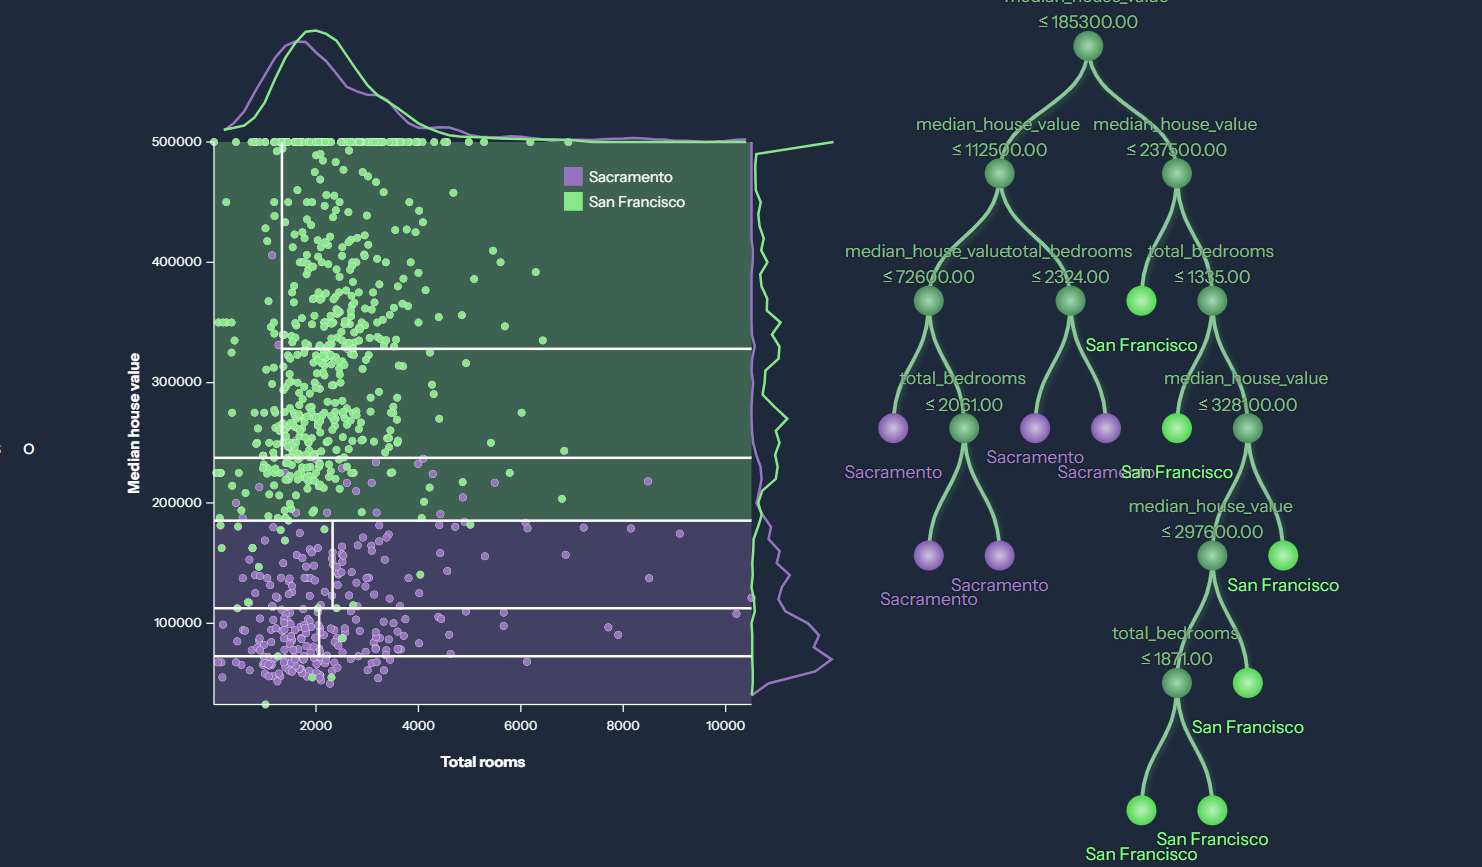
\includegraphics[width=0.4\textwidth]{treeCut.png}
    \caption{Construção da árvore mostra a divisão do espaço 2d}
    \label{fig:minha_imagem}
\end{figure}

Para esta visualização, selecionamos duas variáveis preditoras que permitem a representação em um espaço bidimensional: median\_house\_value e total\_bedrooms. A visualização começa exibindo o espaço inteiro sem divisões, acompanhada de um texto introdutório. A cada rolagem do usuário, é aplicado um corte no scatterplot e são criados dois ramos na árvore, processo que se repete até que toda a árvore de decisão esteja construída. A estrutura da árvore é representada por meio de um dendograma interativo implementado com D3.js [4], o que permite acompanhar visualmente, em paralelo, a segmentação dos dados e o crescimento da árvore. O objetivo final desse gráfico é ilustrar a correspondência entre os cortes no espaço dos dados e a estrutura lógica da árvore de decisão.


\subsection{Previsão interativa}

\begin{figure}[h]
    \centering
    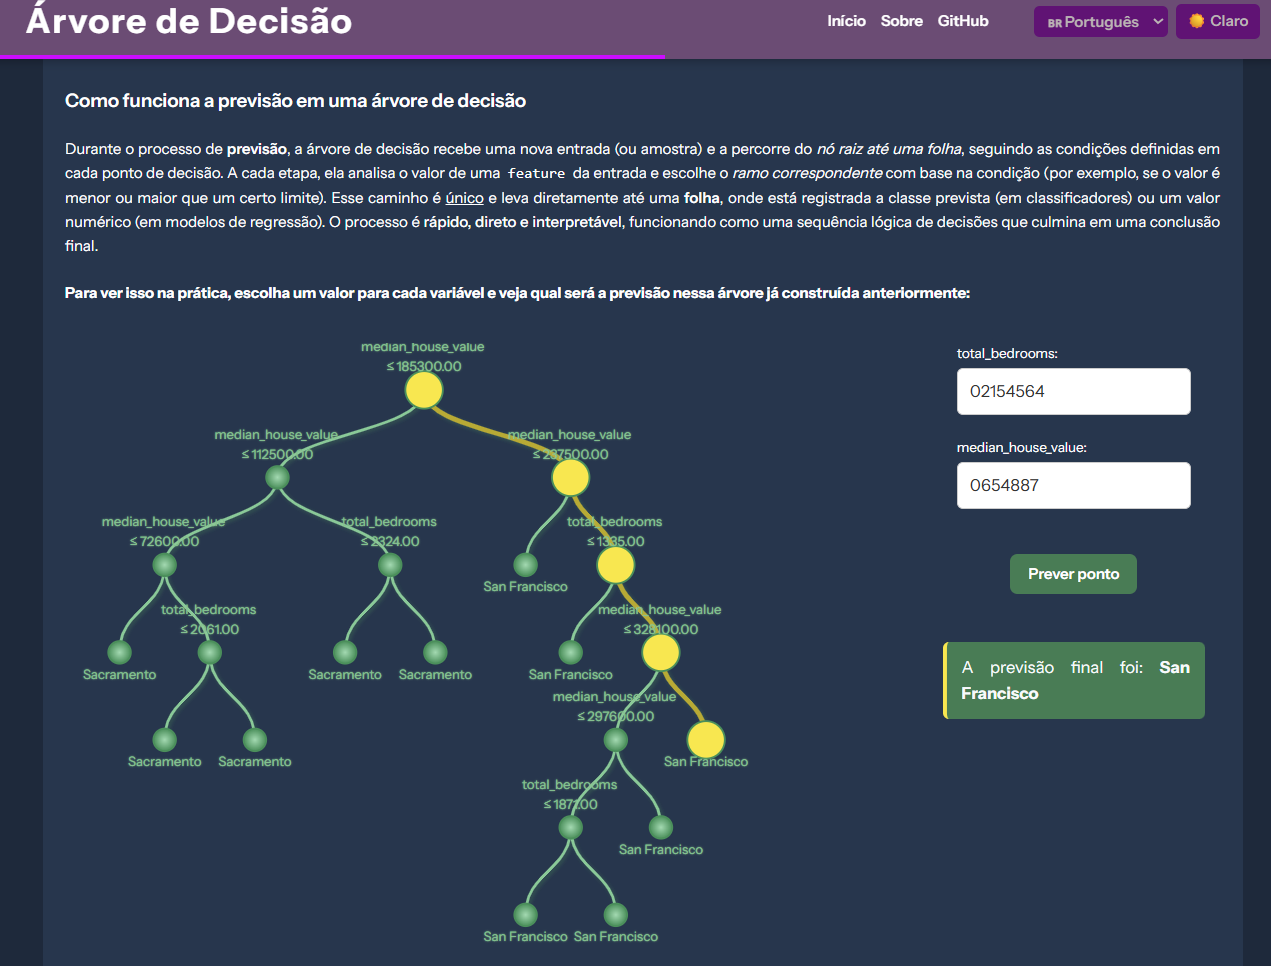
\includegraphics[width=0.35\textwidth]{prev.png}
    \caption{Previsão com interatividade para o usuário}
    \label{fig:minha_imagem}
\end{figure}

    Com a árvore construída a partir das duas variáveis selecionadas, exibimos sua estrutura completa e incluímos uma interação que permite ao usuário inserir valores para essas variáveis. A partir disso, é possível acompanhar visualmente o caminho percorrido por uma amostra ao "descer" pela árvore, até chegar a uma folha, onde é feita a predição final.
\subsection{Definição e visualização de impureza}
\begin{figure}[h]
    \centering
    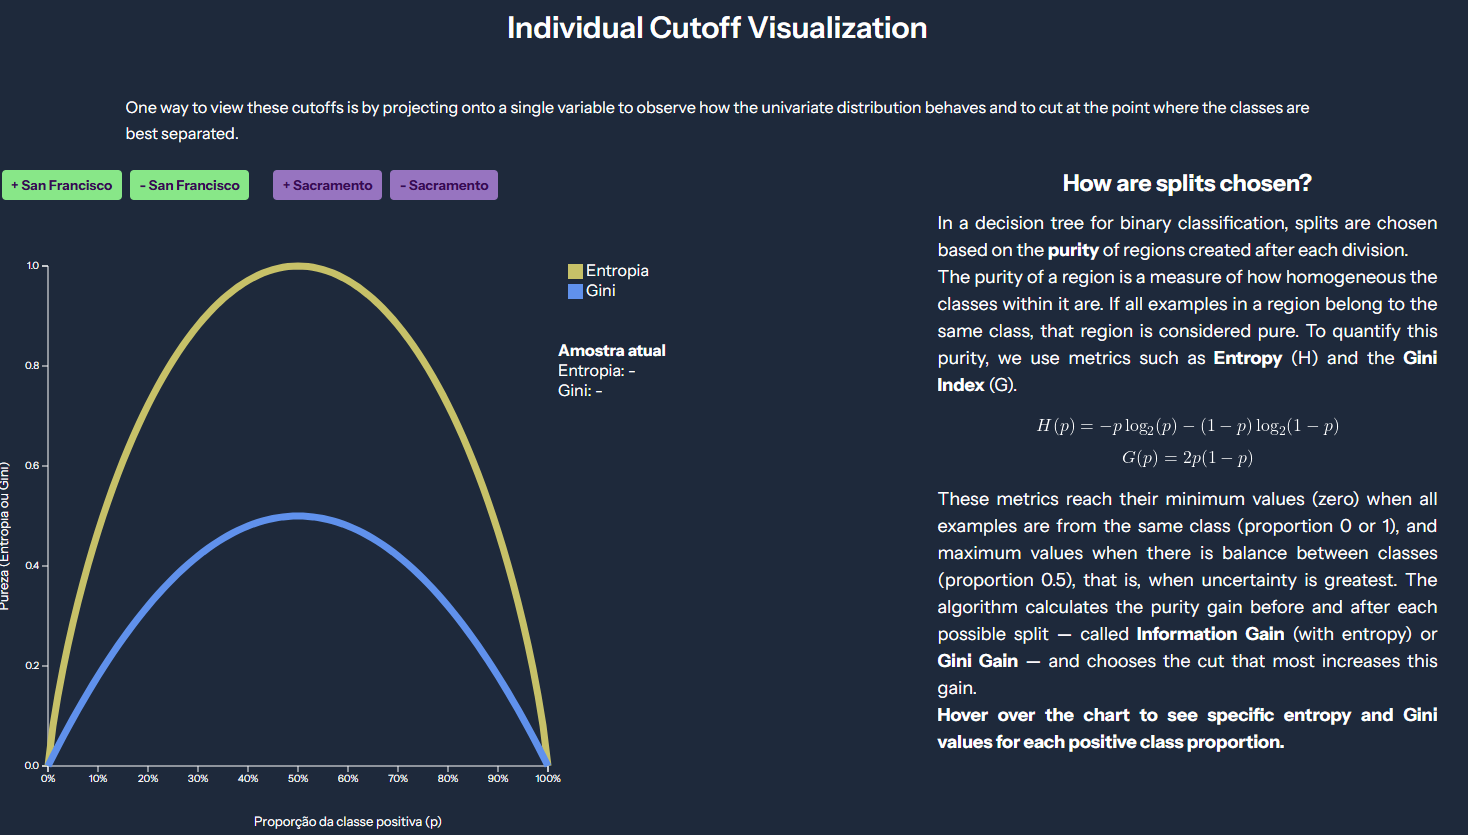
\includegraphics[width=0.35\textwidth]{gini.png}
    \caption{Impureza ao longo da proporção de classe}
    \label{fig:minha_imagem}
\end{figure}
    Com o conceito de corte já apresentado, esta seção tem como objetivo explicar a impureza das regiões divididas. Para isso, introduzimos as métricas de entropia e índice de Gini, que medem a impureza de uma região com base na proporção de classes presentes nas subregiões formadas após a divisão. Além disso, o gráfico nesta seção permite ao usuário interagir adicionando ou removendo amostras das classes 'San Francisco' ou 'Sacramento', observando como essas alterações impactam as medidas de impureza.

    
\subsection{Escolha do melhor corte}

\begin{figure}[h]
    \centering
    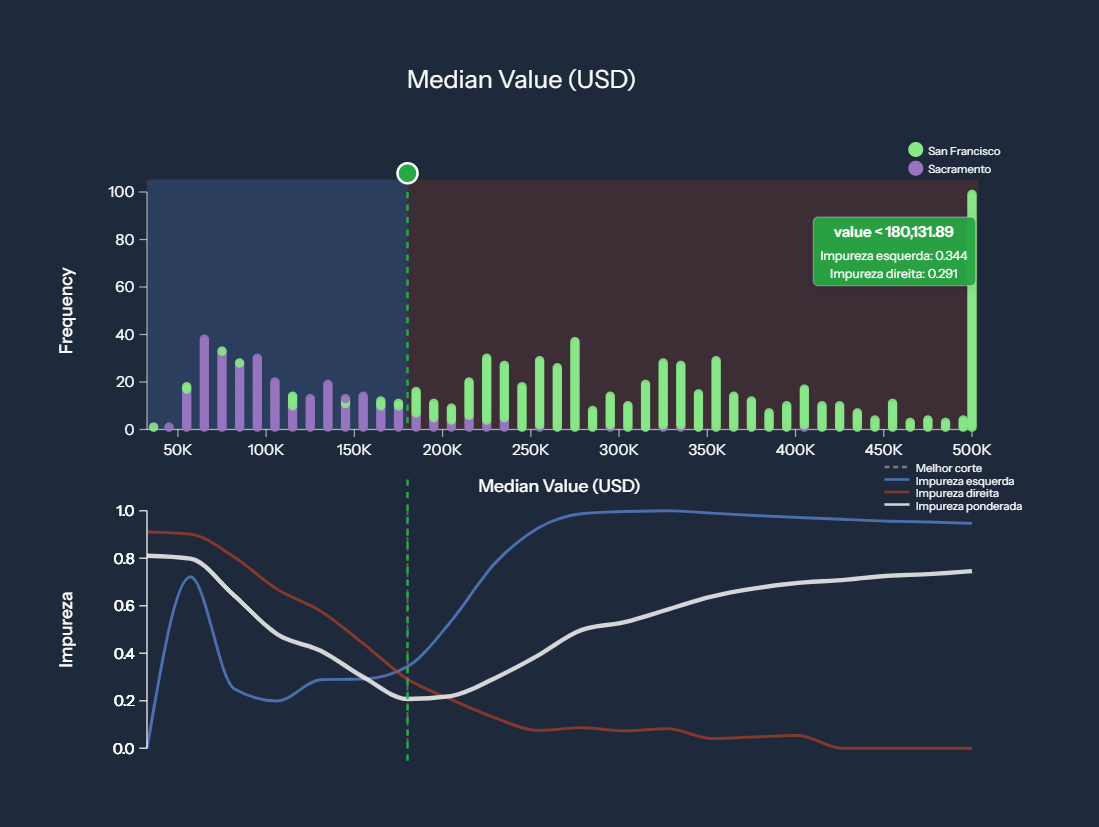
\includegraphics[width=0.35\textwidth]{unicut.png}
    \caption{Cálculo de impureza para vários limiares}
    \label{fig:minha_imagem}
\end{figure}
   Nesta etapa, buscamos ilustrar como o algoritmo de árvore de decisão escolhe o ponto de corte ideal para uma variável preditora. A análise é feita com base na avaliação da impureza nas regiões resultantes após cada possível divisão.
    A visualização associada permite explorar interativamente como a impureza se comporta ao longo do eixo da variável. O objetivo é encontrar o ponto que minimiza a impureza ponderada, ou seja, que resulta em subconjuntos mais homogêneos. Além disso, a interação permite ao usuário ajustar o limiar de corte e observar o impacto dessa escolha nas métricas de impureza.
    Essa abordagem reforça a compreensão intuitiva de como funciona o processo de divisão em uma árvore de decisão.
\subsection{Árvore completa e com poda}

\begin{figure}[h]
    \centering
    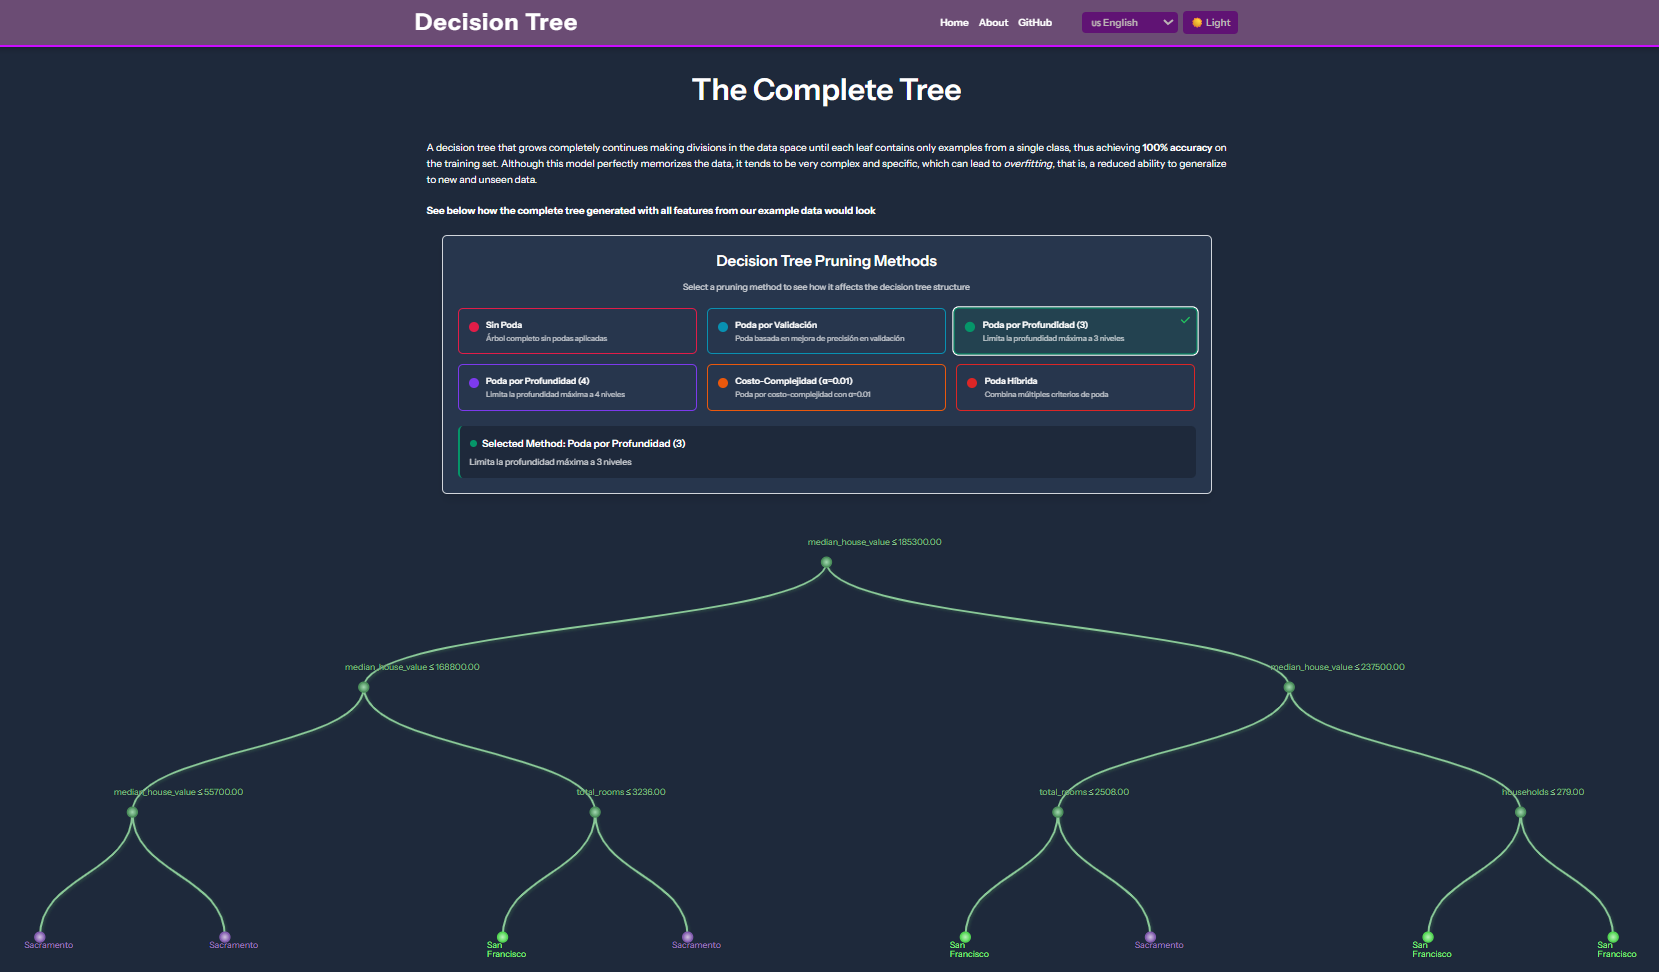
\includegraphics[width=0.4\textwidth]{treePrun.png}
    \caption{Exibição da árovore com poda por profundidade (3)}
    \label{fig:minha_imagem}
\end{figure}

Por fim, a última seção da visualização apresenta diferentes configurações de árvores de decisão, com foco na comparação entre uma árvore totalmente expandida (completa) e versões podadas. A primeira configuração exibida é a chamada árvore completa, na qual o modelo cresce até atingir pureza total, ou seja, classifica corretamente todas as amostras do conjunto de treino. Apesar de parecer ideal, essa abordagem leva a um overfitting severo: o modelo se ajusta excessivamente aos dados de treinamento, capturando ruídos e padrões específicos que não se generalizam. Como resultado, a acurácia em novos dados tende a cair significativamente, mesmo que a acurácia de treino seja de 100\%.

Para contornar esse problema, são exploradas diferentes estratégias de poda. As abordagens disponíveis são:
\begin{itemize}
    \item \textbf{Poda por profundidade}: limita a profundidade máxima da árvore, ignorando subdivisões abaixo de um certo nível. No projeto, é possível aplicar podas com profundidade máxima 3 ou 4.

\item \textbf{Poda por complexidade}: essa técnica avalia o equilíbrio entre a complexidade da árvore e sua capacidade de generalização. Um parâmetro de regularização $\alpha$ é usado para penalizar árvores mais complexas, promovendo estruturas mais simples que ainda tenham bom desempenho, ou seja prefere árvores com poucos ramos e pouca profundidade que tenham bom desempenho. No site, disponibilizamos uma versão com $\alpha$ = 0.01.

\item \textbf{Poda por validação}: a árvore é inicialmente construída de forma completa, e os ramos menos relevantes são eliminados com base no desempenho observado em um conjunto separado. Essa técnica visa preservar apenas as divisões que realmente contribuem para a performance em dados não vistos.

\item \textbf{Poda híbrida}: combina as abordagens anteriores, ajustando a árvore com base em múltiplos critérios (profundidade, complexidade e validação) para alcançar um equilíbrio mais robusto entre simplicidade e capacidade preditiva.
\end{itemize}

Essas estratégias demonstram visualmente como diferentes formas de poda influenciam a forma e o desempenho da árvore, ressaltando a importância do controle da complexidade em modelos de aprendizado supervisionado.

\section{Resultados e Discussão}
As visualizações interativas desenvolvidas funcionam como uma ferramenta didática, facilitando a compreensão do funcionamento das Árvores de Decisão.

A metodologia ScrollStory mostrou-se particularmente eficaz ao guiar o usuário pelo processo de construção e interpretação do modelo. Ao manter a visualização gráfica no centro da tela enquanto o conteúdo textual avança com a rolagem, o foco visual é preservado, permitindo uma experiência de aprendizagem fluida e intuitiva. Isso proporciona uma melhor assimilação de como a árvore realiza classificações.

A interface ilustra claramente como as variáveis do conjunto de dados são utilizadas para gerar pontos de divisão e ramificações, com o objetivo de maximizar a pureza das amostras em cada folha da árvore. Conceitos fundamentais como overfitting são incorporados de maneira visual, demonstrando como o excesso de complexidade pode prejudicar a generalização do modelo, mesmo que ele tenha desempenho perfeito nos dados de treinamento.

Os principais conceitos de aprendizado de máquina abordados ao longo da visualização incluem:

\begin{itemize}
    \item Classificação: o problema central da visualização é categorizar (classificar) casas como pertencentes a 
    Sacramento ou São Francisco, uma tarefa de classificação binária.
    \item Características (Features): as variáveis do conjunto de dados (total\_rooms, total\_bedrooms, households, median\_house\_value)
    são apresentadas como "features" ou "preditores", que o modelo usa para tomar decisões.
    \item Divisões e Limites: demonstra como uma árvore de decisão identifica "limites" 
    nos dados, que são os "pontos de divisão".
    \item Ramificações: as decisões da árvore são representadas como "instruções se-então" ou "ramificações", que dividem os dados em dois "ramos" com base em um valor.
    \item Pureza e Ganho de Informação: a visualização tem como objetivo mostrar como as 
    decisões são tomadas para tornar os ramos resultantes o mais "homogêneos" ou "puros" possível. 
    \item Overfitting: assim como as referências, buscamos contextualizar o problema do overfitting, 
    onde o modelo aprende detalhes irrelevantes dos dados de treinamento, resultando em desempenho menos ideal em dados não vistos.
\end{itemize}

Em síntese, a visualização permite que o usuário compreenda de forma intuitiva e interativa como as Árvores de Decisão operam, promovendo não apenas a aprendizagem conceitual, mas também o entendimento visual do processo de classificação, da formação das divisões e das consequências do sobreajuste.

\section{Trabalhos Futuros}
Para aprimorar esta ferramenta educacional e abordar as limitações intrínsecas das árvores de decisão simples, diversas direções para trabalhos futuros podem ser exploradas:
\begin{itemize}
    \item \textbf{Controle de poda interativo}: implementar um recurso onde o usuário possa escolher parâmetros de profundidade e pureza para realizar a poda da árvore.
    \item \textbf{Extensão para Random Forests}: desenvolver módulos que demonstrem como múltiplas árvores de decisão (random forests) podem ser combinadas para superar a instabilidade e alta variância de uma única árvore.
    \item \textbf{Adaptação para Regressão}: estender a visualização para explicar como as árvores de decisão são usadas em problemas de regressão, não apenas classificação.
    \item \textbf{Entrada de dados customizados pelo usuário}: permitir que o usuário envie seu próprio dataset, e a interface construa a árvore de classificação e, opcionalmente, realiza a poda.
\end{itemize}
Essas extensões contribuiriam significativamente para a ferramenta, tornando-a ainda mais robusta e abrangente para o ensino de conceitos de aprendizado de máquina.

\begin{thebibliography}{00}
\bibitem{r2d3} R2D3. \textit{A Visual Introduction to Machine Learning}. Disponível em: \url{http://www.r2d3.us/visual-intro-to-machine-learning-part-1/}. Acesso em: Jun. 2025.
\bibitem{mlu} MLU. \textit{Decision Trees – Explained Visually}. Disponível em:

\url{https://mlu-explain.github.io/decision-tree/}. Acesso em: Jun. 2025.

\bibitem{californiaHousing} Kaggle. \textit{California Housing Prices}. Disponível em: \url{https://www.kaggle.com/datasets/camnugent/california-housing-prices/data}. Acesso em: Maio 2025.

\bibitem{Dendograma D3} D3.js. \textit{Dendograma D3}. Disponível em: \url{https://d3-graph-gallery.com/dendrogram}.

\url{https://www.data-to-viz.com/graph/dendrogram.html}
Acesso em: Jun. 2025.

\end{thebibliography}

\end{document}